\documentclass[
	fontsize=12pt,          % default font size 12pt
	paper=a4,               % DIN A4 page format
	numbers=noenddot,       % remove dots behind chapter numbers (e.g. 1.5 not 1.5.)
	listof=totoc,           % add list of figures, tables, etc. to ToC
	listof=entryprefix,     % add entry name to figures, tables, etc.
	listof=nochaptergap,    % no chapter gap for figures, tables, etc.
	bibliography=totoc,     % add bibliography to ToC but without a chapter number
	parskip=half,           % half line spacing between paragraphs
	openany                 % chapters can start on any page
]{scrbook}

\include{../../for_latex/preamble}

\begin{document}

\begin{titlepage}
	\pagestyle{empty}

	% HFU Logo
	\begin{flushright}
		\begin{figure}[ht]
			\flushright
			
\includegraphics[height=2cm]{../../for_latex/hfu}
		\end{figure}
	\end{flushright}

	\begin{center}
		\vspace{3cm}

		{\fontsize{22}{22} \selectfont \textbf{Blatt 2}}\\[5mm]
		{\fontsize{18}{18} \selectfont Grundlagen der IT-Sicherheit}

		\vspace{12cm}

		{\fontsize{14}{14} \selectfont Luis Staudt}
	\end{center}
\end{titlepage}

% ############################################################################
% CONTENT STARTS HERE
% ############################################################################

\chapter*{Aufgabe 1: Das Smartphone mit dem WLAN und dem VoIP-Server verbinden}

\section*{c) Verbindungstest mit Nummer 1234}
Hello World

\section*{d) Anruf bei Nummer 999}
Input: Hallo\\
Output: Hallo

Input: Wer spricht da\\
Output: Wer spricht da

Es wird genau das ausgegeben was eingegeben wird.
Die Nummer 999 ist ein Echo-Dienst, der die eigene Sprache zurückspielt.


\chapter*{Aufgabe 2: Das WLAN abhören (Schritt 1)}

\section*{c) airodump-ng}

\begin{figure}[h]
	\centering
	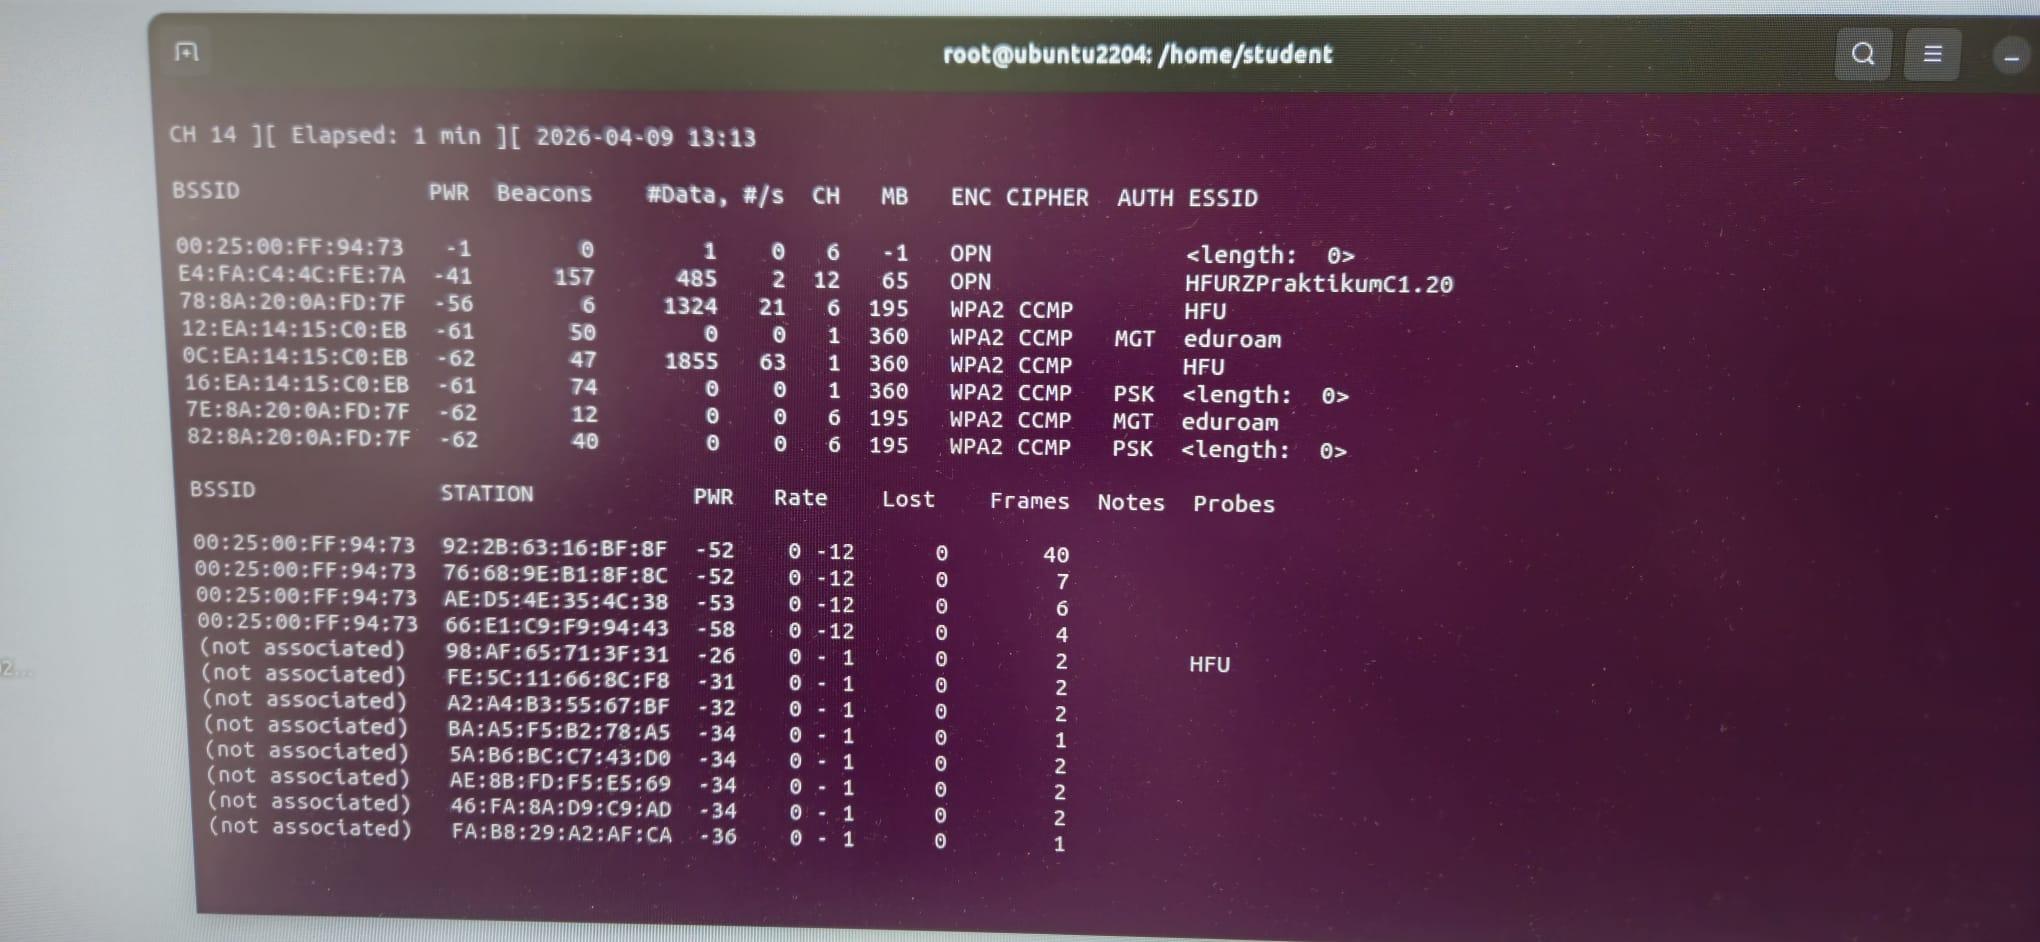
\includegraphics[width=\textwidth]{images/airodump_all_channels}
	\caption{Ausgabe von airodump-ng auf allen Kanälen}
\end{figure}

Das Netzwerk HFURZPraktikumC1.20 wird auf Kanal 12 ausgestrahlt.
Aus der Ausgabe von airodump-ng lässt sich außerdem ablesen: die BSSID des Access Points, die Verschlüsselung (OPN, also offen/unverschlüsselt), die Signalstärke (PWR), die Anzahl der Beacons und Datenpakete sowie die verbundenen Stationen.
Die WLAN-Stationen auf allen Kanälen sind sichtbar, weil airodump-ng im Monitor-Modus automatisch zwischen den Kanälen wechselt (Channel Hopping), um alle aktiven Netzwerke zu erfassen.


\chapter*{Aufgabe 3: Das WLAN abhören (Schritt 2)}

\section*{b) Paketaufzeichnung mit airodump-ng}

\begin{figure}[h]
	\centering
	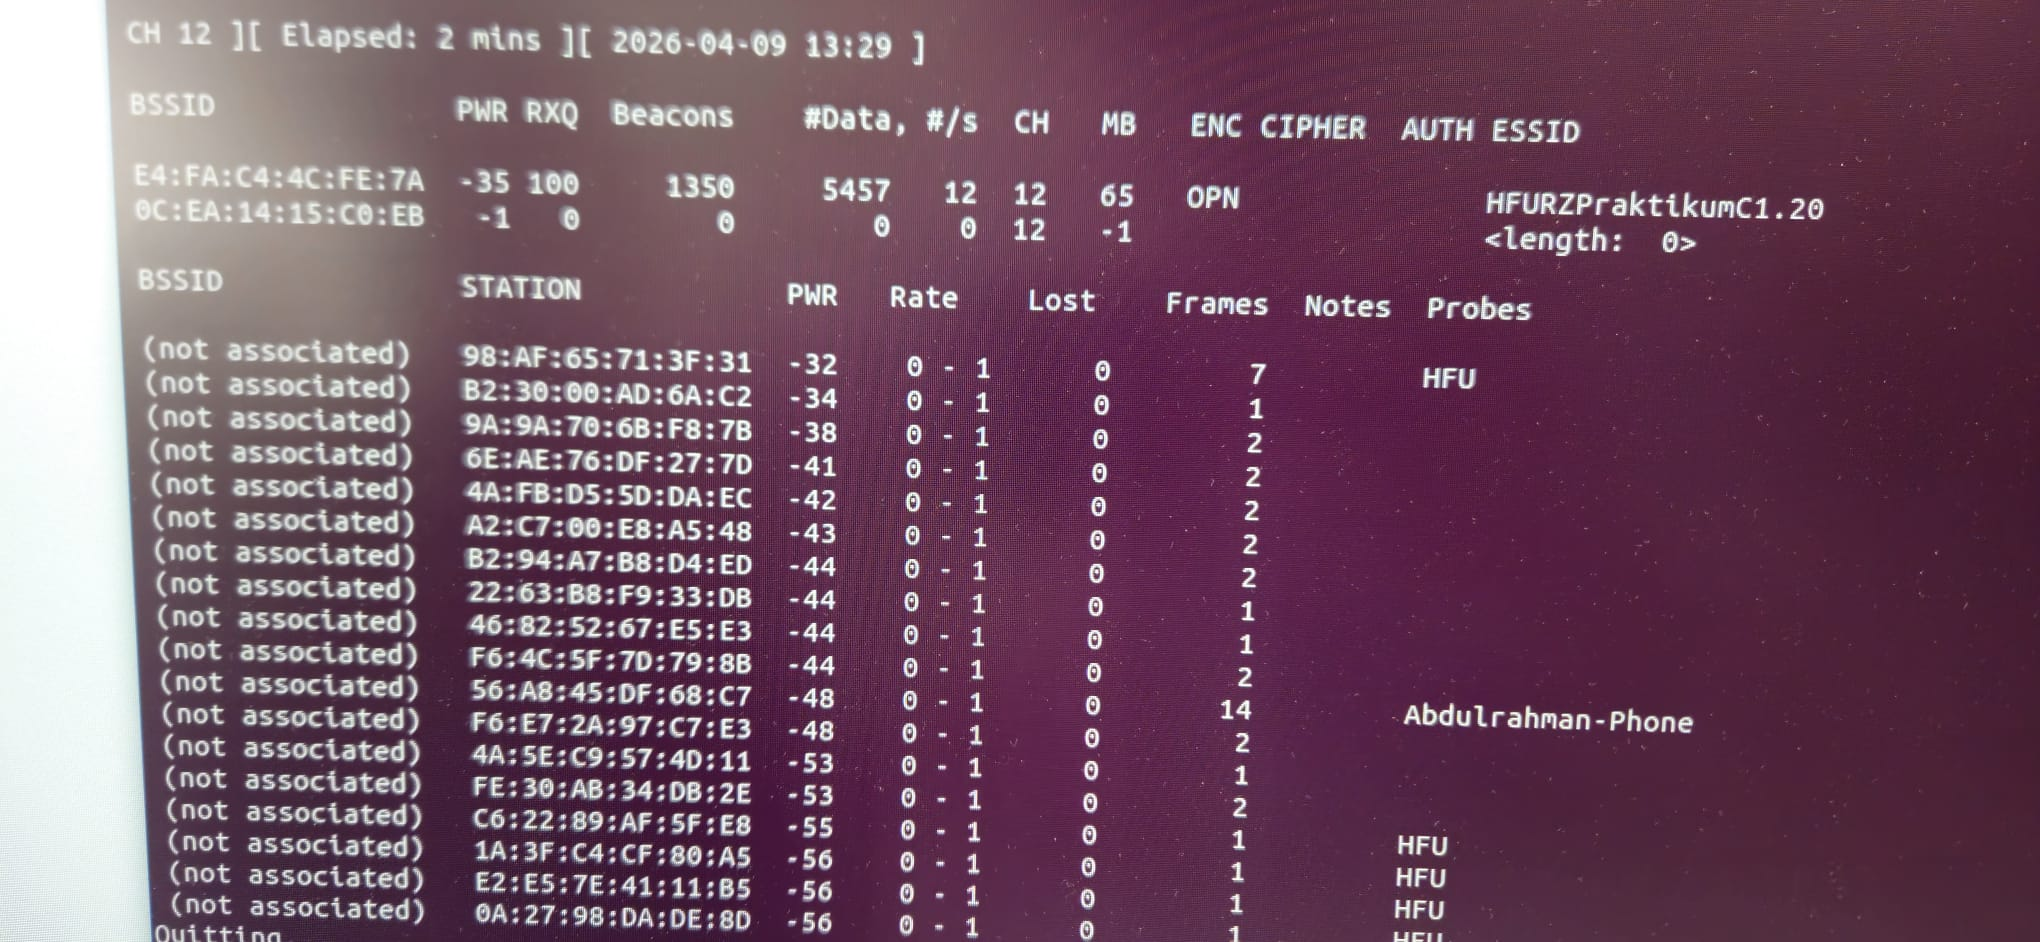
\includegraphics[width=\textwidth]{images/airodump_channel12}
	\caption{Ausgabe von airodump-ng auf Kanal 12 mit Paketaufzeichnung}
\end{figure}

Mit dem Befehl \texttt{airodump-ng -{}-channel 12 -{}-write capture-01 wlan0mon} wurde der Datenverkehr auf Kanal 12 aufgezeichnet und in die Datei capture-01 geschrieben.

\section*{d) Warum den richtigen Kanal einstellen?}
Ohne die Einstellung auf den richtigen Kanal wechselt airodump-ng ständig zwischen allen Kanälen (Channel Hopping).
Dabei werden nur Bruchteile des Datenverkehrs auf jedem Kanal erfasst, da die Karte die meiste Zeit auf anderen Kanälen lauscht.
Um ein vollständiges Mitschneiden des VoIP-Anrufs zu ermöglichen, muss die Karte dauerhaft auf dem Kanal des Zielnetzwerks verbleiben.


\chapter*{Aufgabe 4: Den Anruf aus den aufgezeichneten Daten extrahieren}

\section*{c) Screenshot von Wireshark}

\begin{figure}[h]
	\centering
	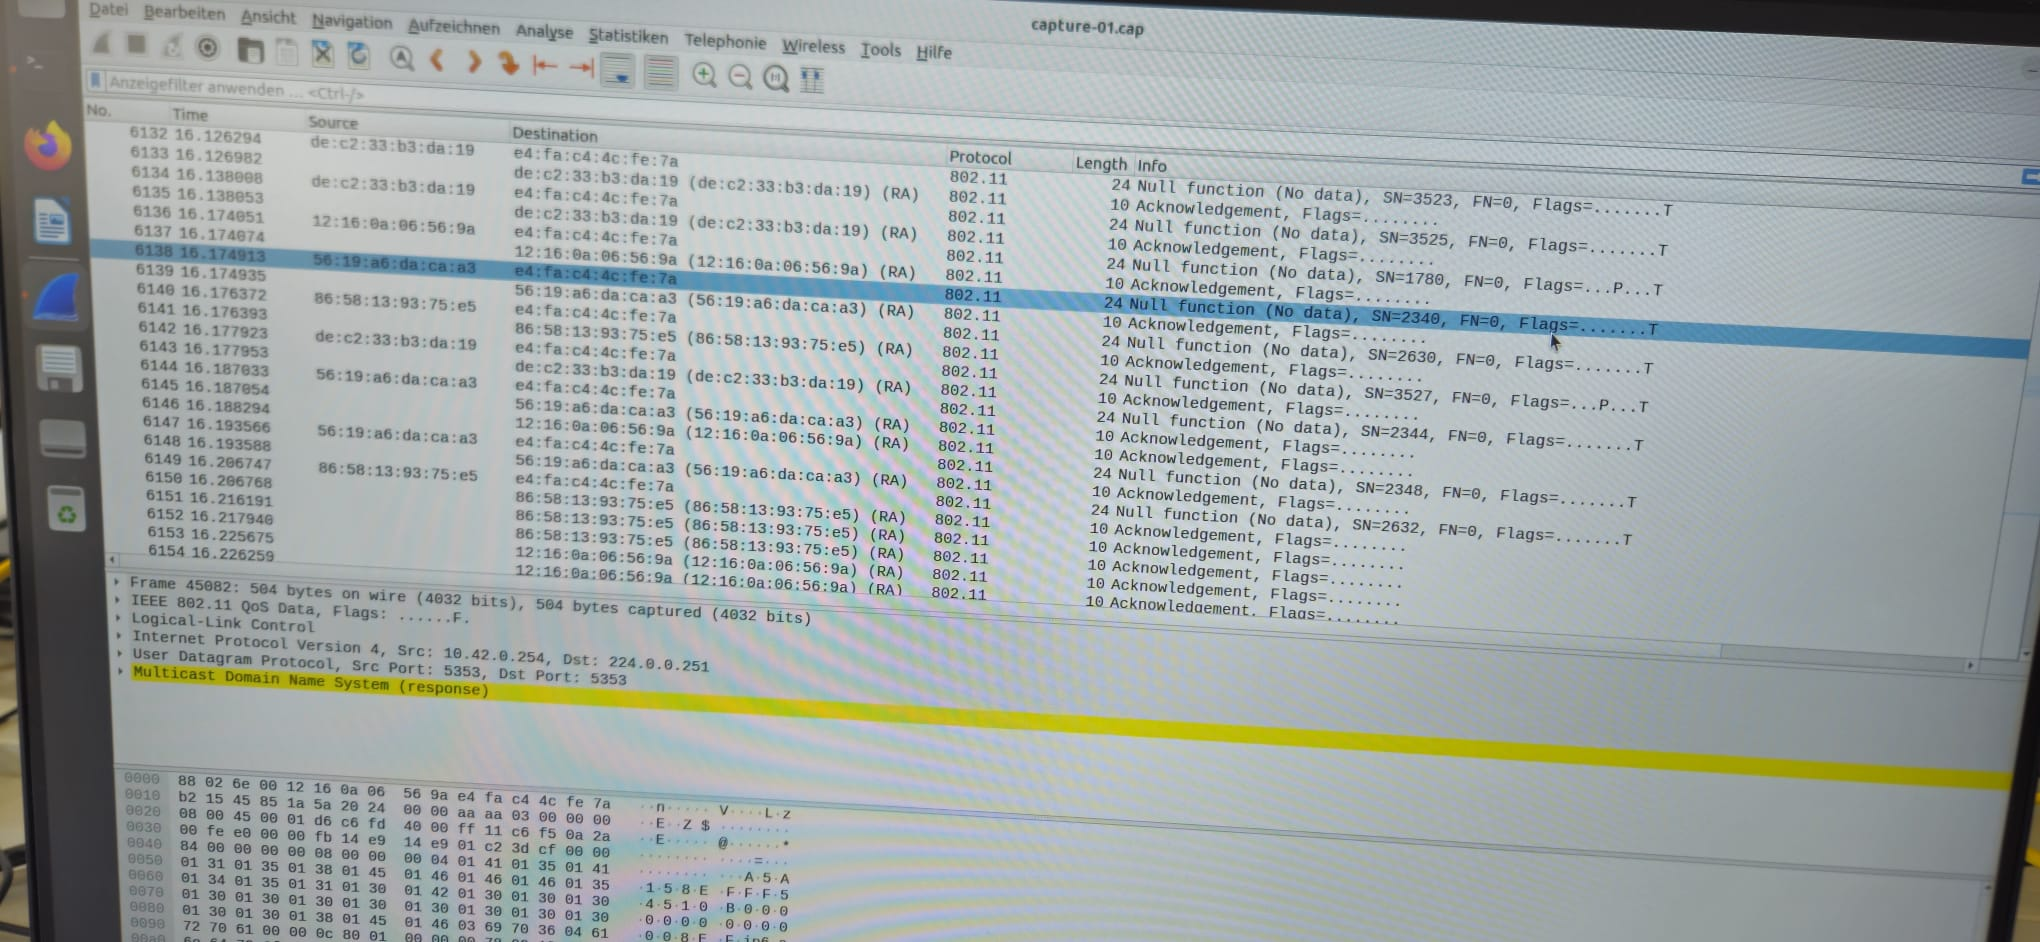
\includegraphics[width=\textwidth]{images/wireshark_packets}
	\caption{Wireshark zeigt die aufgezeichneten Pakete}
\end{figure}

Wireshark zeigt die einzelnen aufgezeichneten Netzwerkpakete mit Zeitstempel, Quell- und Zieladresse, Protokoll und weiteren Details an.
Darunter befinden sich unter anderem IEEE 802.11 WLAN-Frames, SIP-Signalisierungspakete und RTP-Audiodaten des VoIP-Anrufs.

\section*{d) Telefonate anzeigen und abspielen}

\begin{figure}[h]
	\centering
	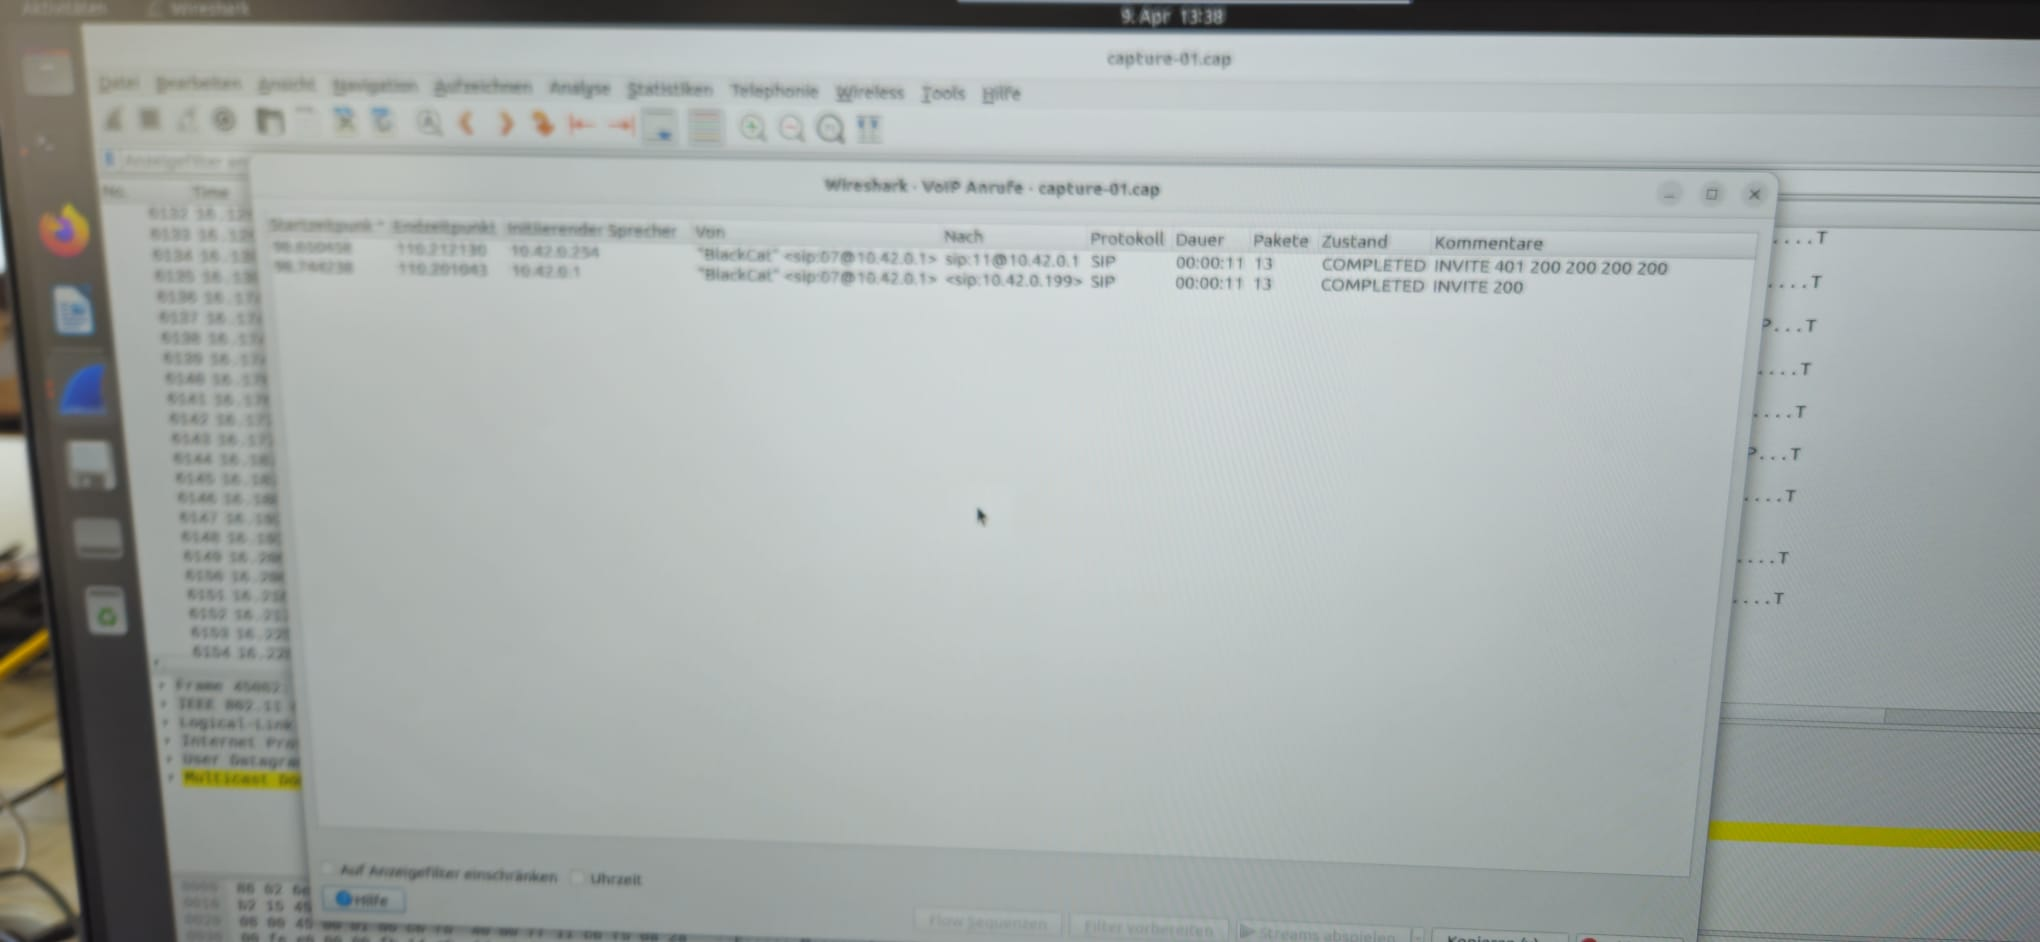
\includegraphics[width=\textwidth]{images/wireshark_voip_calls}
	\caption{Wireshark VoIP-Anrufe}
\end{figure}

Über das Menü Telefonie $\rightarrow$ VoIP-Anrufe lassen sich die aufgezeichneten Telefonate anzeigen.
Es sind mehr als nur der eigene Anruf sichtbar, da im offenen WLAN der gesamte Datenverkehr aller Teilnehmer mitgeschnitten wurde.
Jeder VoIP-Anruf anderer Nutzer im selben Netzwerk wurde ebenfalls aufgezeichnet.

\section*{e) Wellenform des Anrufs}

\begin{figure}[h]
	\centering
	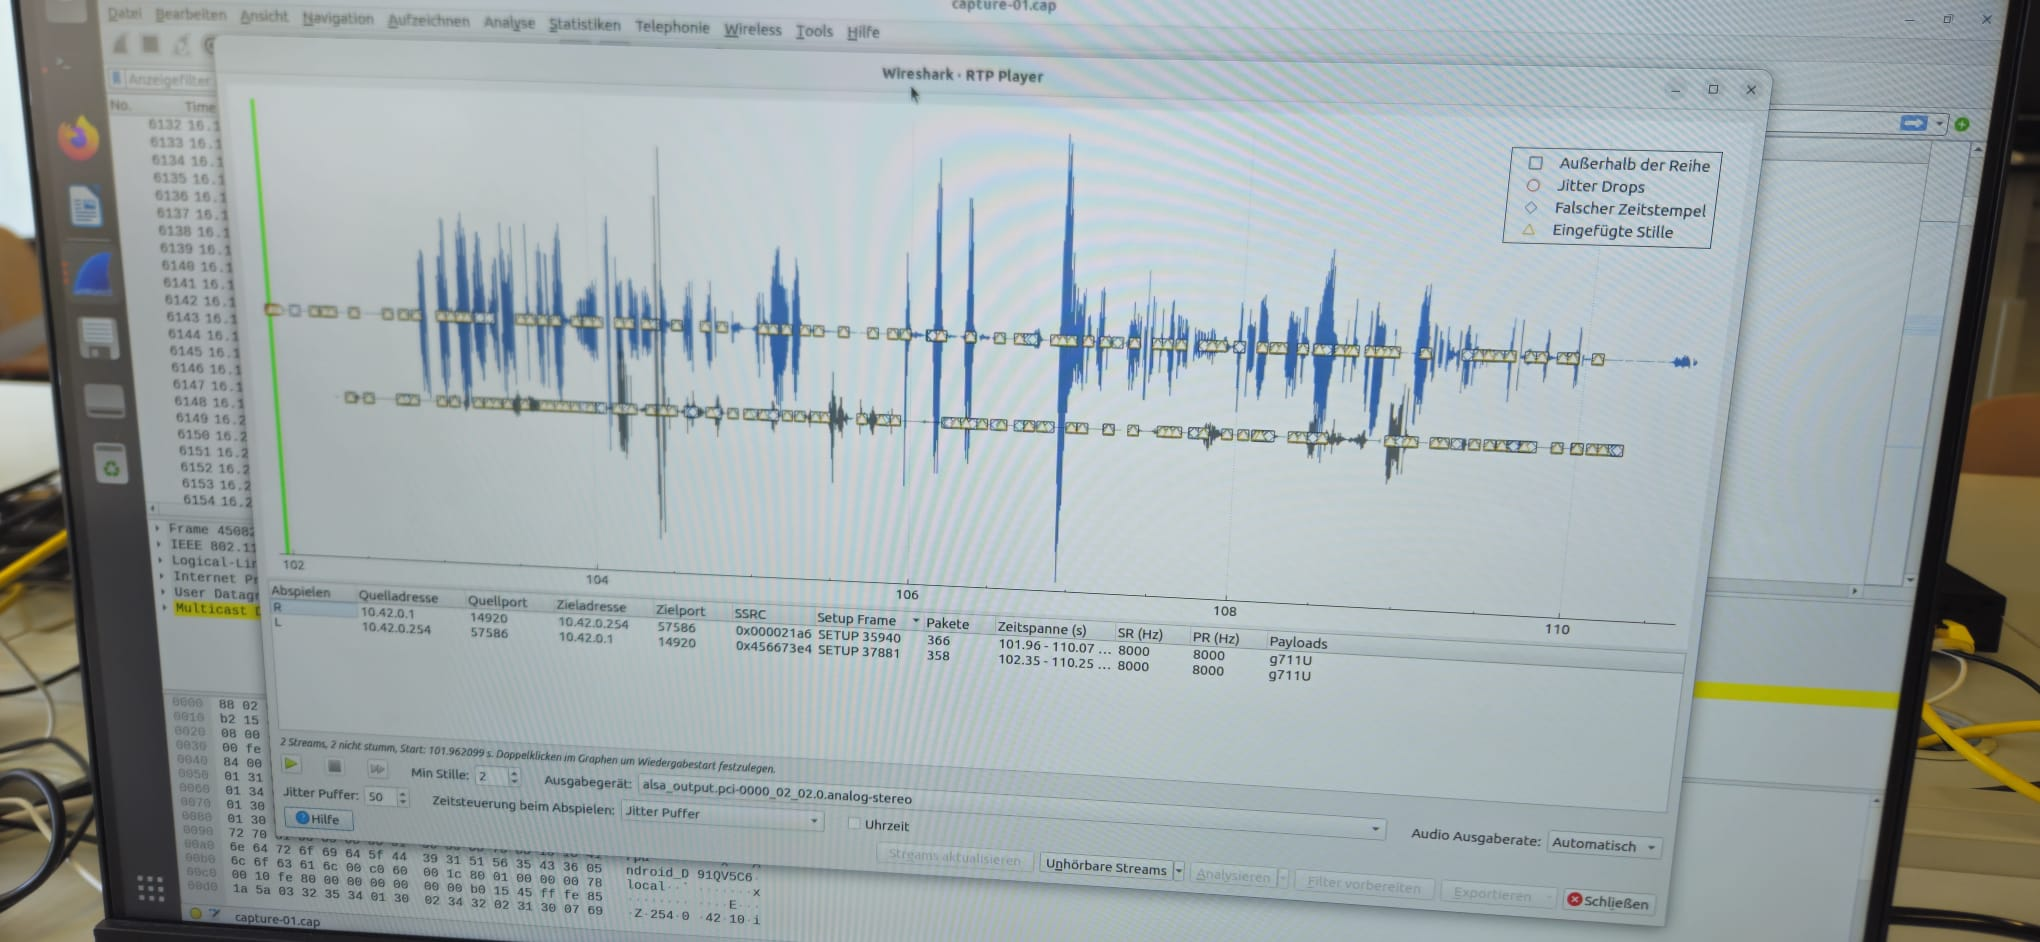
\includegraphics[width=\textwidth]{images/wireshark_waveform}
	\caption{Wellenform des abgespielten VoIP-Anrufs im RTP-Player}
\end{figure}


\chapter*{Aufgabe 5: Wie könnten Sie sich schützen?}

\section*{a) Verletztes Schutzziel und Bedrohung}
Das Schutzziel der Vertraulichkeit wurde verletzt.
Die Bedrohung ist Information Disclosure: Der Inhalt des VoIP-Telefonats konnte von einem unbefugten Dritten mitgehört werden, da das WLAN unverschlüsselt war und die Sprachdaten unverschlüsselt per RTP übertragen wurden.

\section*{b) Schutzmaßnahmen}
Es gibt mehrere Möglichkeiten, sich vor einem solchen Angriff zu schützen:
\begin{itemize}
	\item WLAN-Verschlüsselung: Verwendung von WPA2 oder WPA3 statt eines offenen WLANs.
	Dadurch kann der Datenverkehr nicht einfach mitgelesen werden.
	\item VoIP-Verschlüsselung: Nutzung von SRTP (Secure RTP) zur Verschlüsselung der Sprachdaten und TLS/SIPS zur Verschlüsselung der SIP-Signalisierung.
	\item VPN: Nutzung eines VPN-Tunnels, der den gesamten Datenverkehr verschlüsselt, unabhängig davon ob das WLAN selbst verschlüsselt ist.
	\item Ende-zu-Ende-verschlüsselte Kommunikation: Verwendung von Messengern mit integrierter Sprachverschlüsselung (z.\,B. Signal) statt unverschlüsseltem SIP/RTP.
\end{itemize}


% ############################################################################
% CONTENT ENDS HERE
% ############################################################################

\end{document}
